\documentclass[11pt, a4paper, titlepage, openright]{article}
% \usepackage[options]{package}

\title{\LARGE Scientific Programming \\ \normalsize Data Fitting Exercise 1}
\author{Armin Halilovic - s0122210}
\date{October 30, 2015}

\usepackage[font=small,labelfont=bf]{caption}
\usepackage{float}
%\floatstyle{boxed}
\restylefloat{figure}
\usepackage{graphicx}
\usepackage{hyperref}
\usepackage{mathtools}
%\usepackage{titlesec}
\usepackage[titletoc, title]{appendix}
\usepackage{listings}
\usepackage{color}

\definecolor{dkgreen}{rgb}{0,0.6,0}
\definecolor{gray}{rgb}{0.5,0.5,0.5}
\definecolor{mauve}{rgb}{0.58,0,0.82}

\lstset{frame=tb,
  language=C++,
  aboveskip=3mm,
  belowskip=3mm,
  showstringspaces=false,
  columns=flexible,
  basicstyle={\footnotesize\ttfamily},
  numbers=none,
  numberstyle=\tiny\color{gray},
  keywordstyle=\color{blue},
  commentstyle=\color{dkgreen},
  stringstyle=\color{mauve},
  breaklines=true,
  breakatwhitespace=true,
  tabsize=3,
  showstringspaces=false
}

\begin{document}
%%%%%%%%%%%%%%%%%%%%%%%%%%%%%%%%%%%%%%%%%
% University Assignment Title Page
% LaTeX Template
% Version 1.0 (27/12/12)
%
% This template has been downloaded from:
% http://www.LaTeXTemplates.com
%
% Original author:
% WikiBooks (http://en.wikibooks.org/wiki/LaTeX/Title_Creation)
%
% License:
% CC BY-NC-SA 3.0 (http://creativecommons.org/licenses/by-nc-sa/3.0/)
%
% Instructions for using this template:
% This title page is capable of being compiled as is. This is not useful for
% including it in another document. To do this, you have two options:
%
% 1) Copy/paste everything between \begin{document} and \end{document}
% starting at \begin{titlepage} and paste this into another LaTeX file where you
% want your title page.
% OR
% 2) Remove everything outside the \begin{titlepage} and \end{titlepage} and
% move this file to the same directory as the LaTeX file you wish to add it to.
% Then add \input{./title_page_1.tex} to your LaTeX file where you want your
% title page.
%
%%%%%%%%%%%%%%%%%%%%%%%%%%%%%%%%%%%%%%%%%

%----------------------------------------------------------------------------------------
%	PACKAGES AND OTHER DOCUMENT CONFIGURATIONS
%----------------------------------------------------------------------------------------
\begin{titlepage}

\newcommand{\HRule}{\rule{\linewidth}{0.5mm}} % Defines a new command for the horizontal lines, change thickness here

\center % Center everything on the page

%----------------------------------------------------------------------------------------
%	HEADING SECTIONS
%----------------------------------------------------------------------------------------

\textsc{\LARGE University of Antwerp}\\[1.5cm] % Name of your university/college
\textsc{\Large }\\[4cm] % Major heading such as course name
\textsc{\Large Scientific Programming}\\[0.5cm] % Minor heading such as course title

%----------------------------------------------------------------------------------------
%	TITLE SECTION
%----------------------------------------------------------------------------------------

\HRule
{ \huge \bfseries Second Session \\ \Large{Exercise 2}}\\ % Title of your document
\HRule \\[1.5cm]

%----------------------------------------------------------------------------------------
%	AUTHOR SECTION
%----------------------------------------------------------------------------------------

\begin{minipage}{0.4\textwidth}
\begin{flushleft} \large
Armin Halilovic - s0122210 % Your name
\end{flushleft}
\end{minipage}
~
\begin{minipage}{0.4\textwidth}
\begin{flushright} \large
\end{flushright}
\end{minipage}\\[4cm]

% If you don't want a supervisor, uncomment the two lines below and remove the section above
%\Large \emph{Author:}\\
%John \textsc{Smith}\\[3cm] % Your name

%----------------------------------------------------------------------------------------
%	DATE SECTION
%----------------------------------------------------------------------------------------

\vfill % Fill the rest of the page with whitespace
{\large August 22, 2016}\\[3cm] % Date, change the \today to a set date if you want to be precise

%----------------------------------------------------------------------------------------
%	LOGO SECTION
%----------------------------------------------------------------------------------------

%\includegraphics{Logo}\\[1cm] % Include a department/university logo - this will require the graphicx package

%----------------------------------------------------------------------------------------


\end{titlepage}
\onecolumn
\tableofcontents
\newpage
%\twocolumn


\section{Problem}
\section{Using the code}
    All of the C++ code can be found in the "main.cpp" file and in appendix A of this document.
    main.cpp comes accompanied by createImages.sh, which contains all of the neccessary UNIX commands to generate the graph images.
    This file relies on the \href{https://www.gnu.org/software/plotutils/manual/en/html_node/graph.html}{graph} program
    in the GNU plotutils package to plot graphs, so make sure that it is installed.

    To compile and run the program, execute the following commands in the build/ directory:
    \begin{lstlisting}
    cmake ..
    make
    chmod +x ./createImages.sh
    ./data_fitting
    \end{lstlisting}
    All of the graphs should be present in the build/images/ directory. If they are not there, make createImages.sh executable
    with "chmod +x" and run it to create them.

\newpage
\section{Solutions}
\subsection{Polynomial through non equidistant points}
\subsection{Natural cubic spline}
\subsection{Cubic spline with modified conditions}

\section{Conclusion}
    After conducting the interpolations, we can conclude that using a cubic spline is the best way to
    approximate the Runge function, if we had to choose between polynomial and spline interpolation.
    This conforms to what we learned during the lecture on data fitting.



\onecolumn
\appendix
\appendixpage
\addappheadtotoc

\section{main.cpp}
    \lstinputlisting[basicstyle=\scriptsize]{../main.cpp}
    \newpage

%\section{createImages.sh}
%    \lstinputlisting[language=bash, basicstyle=\scriptsize]{../createImages.sh}

\end{document}

/iffalse

\[f(x) = \frac{1}{1 + 25 x^{2}} \ \ x \in [-1, 1] \]
\subsection{Polynomial through equidistant points}
\label{sec:firstpoly}
\begin{lstlisting}
int i = 0, size = 17;
double xi, xa1[size], ya1[size];
for (xi = -1; xi <= 1; xi = xi + ( 2 / (double) 16)) {
    xa1[i] = xi;
    ya1[i] = runge_f(xi);
    i++;
}
\end{lstlisting}
\href{https://www.gnu.org/software/gsl/manual/html_node/1D-Higher_002dlevel-Interface.html#g_t1D-Higher_002dlevel-Interface}{gsl\_spline}
In figure~\ref{fig:runge}, we can see what the Runge function looks like.
\begin{figure}[H]
    \centering
    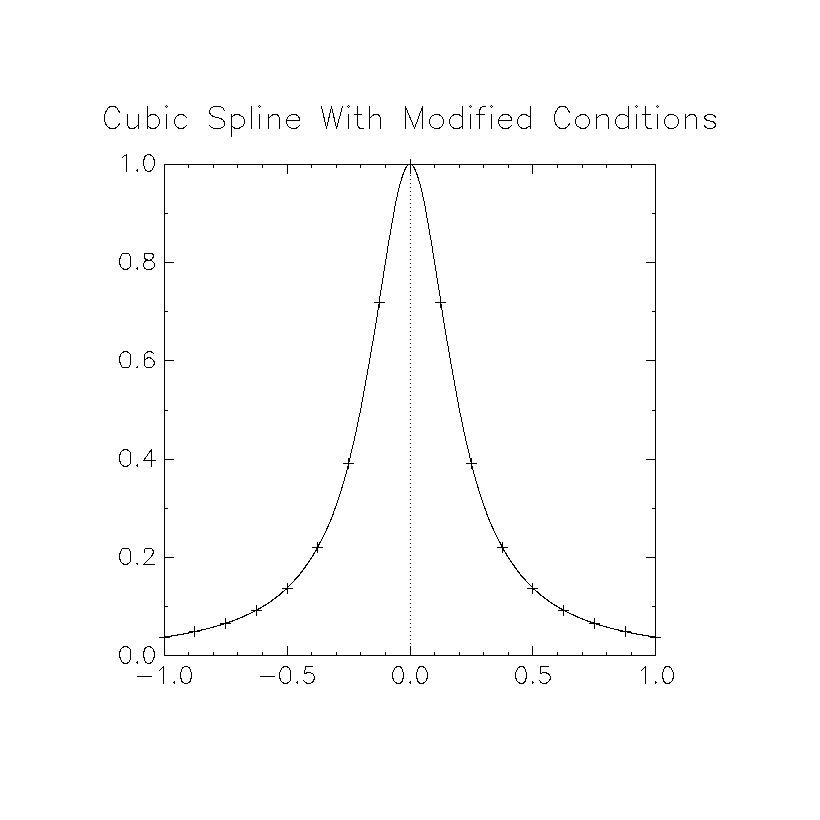
\includegraphics[width=9cm, trim={2cm, 4cm, 2cm, 3cm}, clip]{../images/spline2}
    \caption{Spline interpolation through equidistant points}
    \label{fig:spline2}
\end{figure}
\begin{figure}[H]
    \begin{minipage}[b]{0.49\textwidth}
        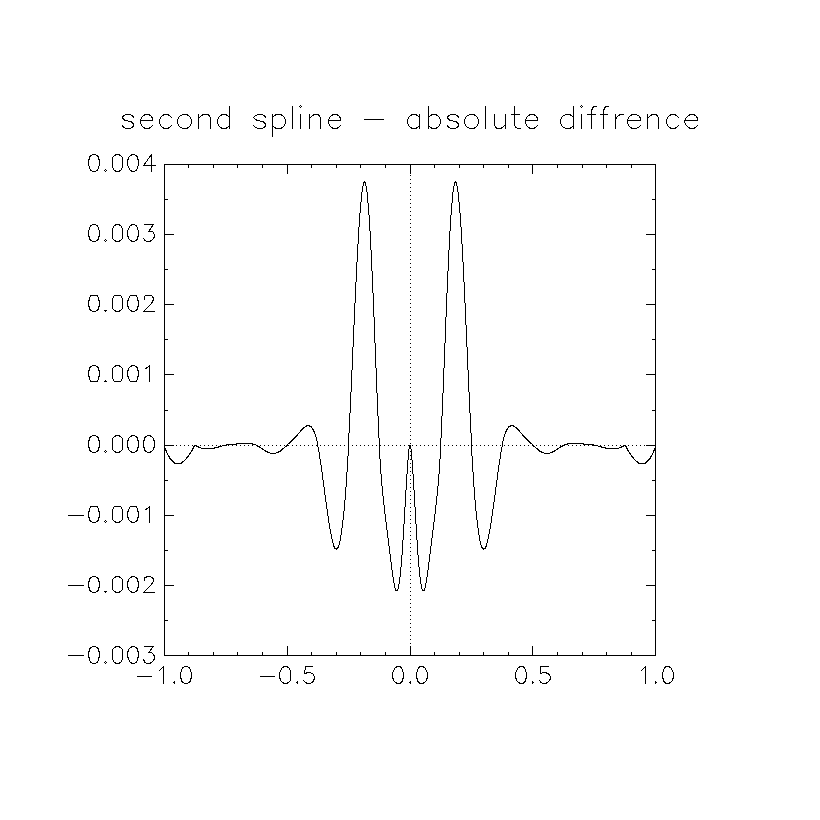
\includegraphics[width=6.5cm, trim={2cm, 4cm, 2cm, 3cm}, clip]{../images/diff4abs}
    \end{minipage}
    \hfill
    \begin{minipage}[b]{0.49\textwidth}
        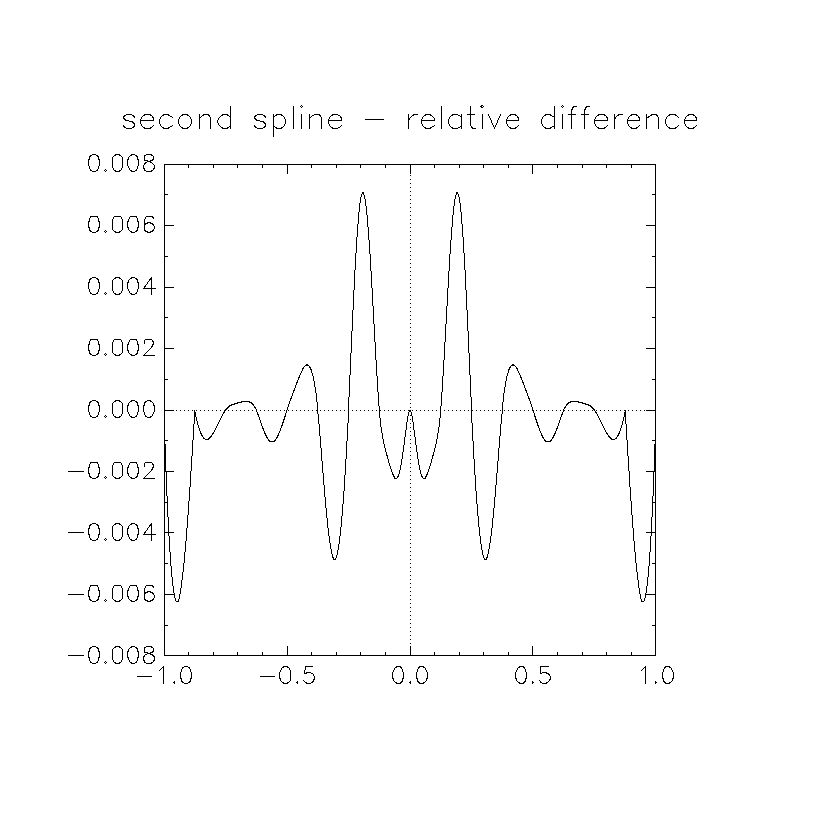
\includegraphics[width=6.5cm, trim={2cm, 4cm, 2cm, 3cm}, clip]{../images/diff4rel}
    \end{minipage}
    \caption{Differences for spline interpolation}
    \label{fig:diff4}
\end{figure}
\bigskip

/fi